\documentclass[noinstructornotes]{ximera}
%handout:  for handout version with no solutions or instructor notes
%handout,instructornotes:  for instructor version with just problems and notes, no solutions
%noinstructornotes:  shows only problem and solutions

%% handout
%% space
%% newpage
%% numbers
%% nooutcomes

%I added the commands here so that I would't have to keep looking them up
%\newcommand{\RR}{\mathbb R}
%\renewcommand{\d}{\,d}
%\newcommand{\dd}[2][]{\frac{d #1}{d #2}}
%\renewcommand{\l}{\ell}
%\newcommand{\ddx}{\frac{d}{dx}}
%\everymath{\displaystyle}
%\newcommand{\dfn}{\textbf}
%\newcommand{\eval}[1]{\bigg[ #1 \bigg]}

%\begin{image}
%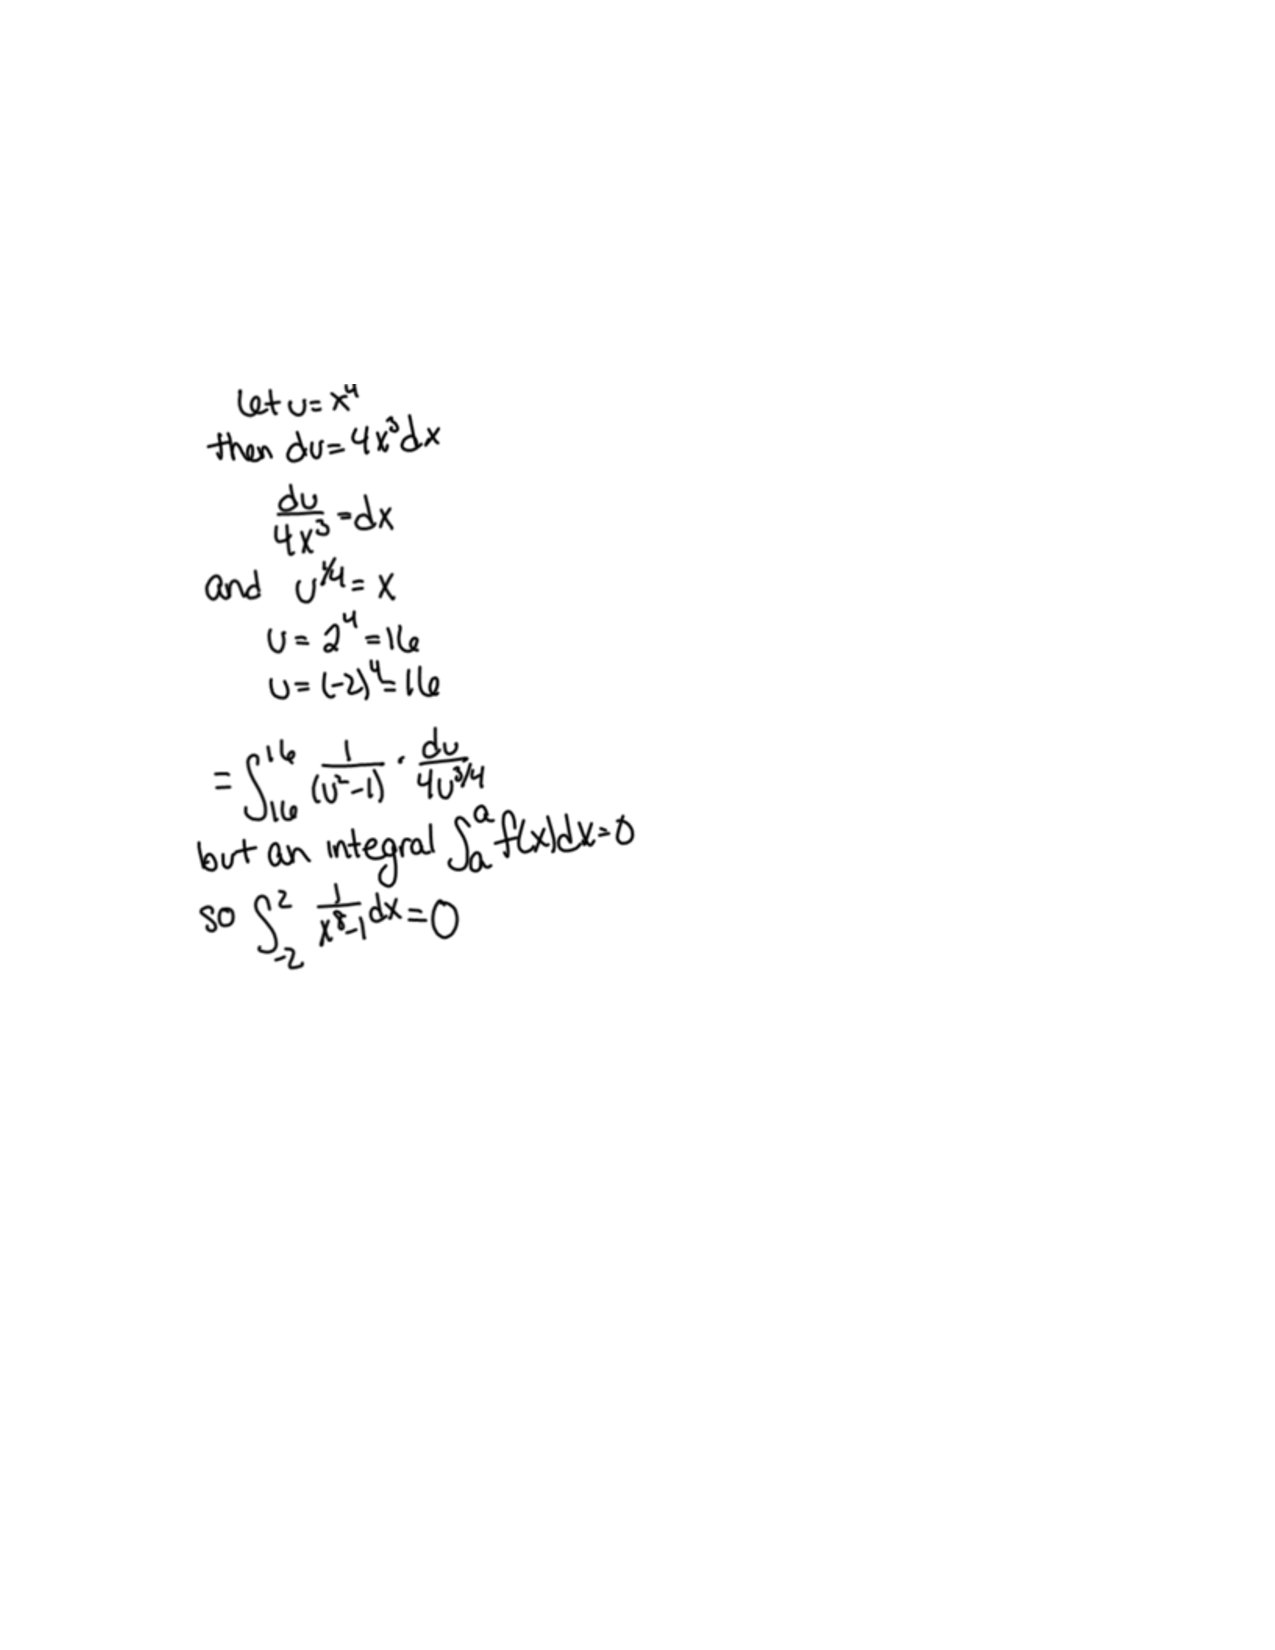
\includegraphics[trim= 170 420 250 180]{Figure1.pdf}
%\end{image}

%add a ``.'' below when used in a specific directory.
\newcommand{\RR}{\mathbb R}
\renewcommand{\d}{\,d}
\newcommand{\dd}[2][]{\frac{d #1}{d #2}}
\renewcommand{\l}{\ell}
\newcommand{\ddx}{\frac{d}{dx}}
\newcommand{\dfn}{\textbf}
\newcommand{\eval}[1]{\bigg[ #1 \bigg]}

\usepackage{multicol}

\renewenvironment{freeResponse}{
\ifhandout\setbox0\vbox\bgroup\else
\begin{trivlist}\item[\hskip \labelsep\bfseries Solution:\hspace{2ex}]
\fi}
{\ifhandout\egroup\else
\end{trivlist}
\fi} %% we can turn off input when making a master document


\title{Section 8.2: Direction fields}  

\begin{document}
\begin{abstract}		\end{abstract}
\maketitle



\begin{comment}

\section{Warm up:}
	Which of the following differential equations are separable?
	\begin{enumerate}
	\item $y' = \frac{ty}{t^2+1}$,
	\item $\frac{dy}{dx} =x^2 \sin (3y) -x^2$,
	\item $y' = t^2 - y$.
	\end{enumerate}

	\begin{freeResponse}
	\begin{enumerate}
	\item Yes, it is separable. $y' = y \cdot \frac{t}{t^2+1}$.
	\item Yes, it is separable. $\frac{dy}{dx} = x^2 \left( \sin(3y)-1 \right)$.
	\item No, it is not separable. $t^2-y$ can not be written in the form $F(t) \cdot G(y)$. 
	\end{enumerate}
	\end{freeResponse}
	
\begin{instructorNotes}

\end{instructorNotes}

\end{comment}






\section{Group work:}



%problem 1
\begin{problem}

 The following is a direction field for the differential equation $\dd[y]{x} = y^2 - x^2$.
	
		\begin{image}
		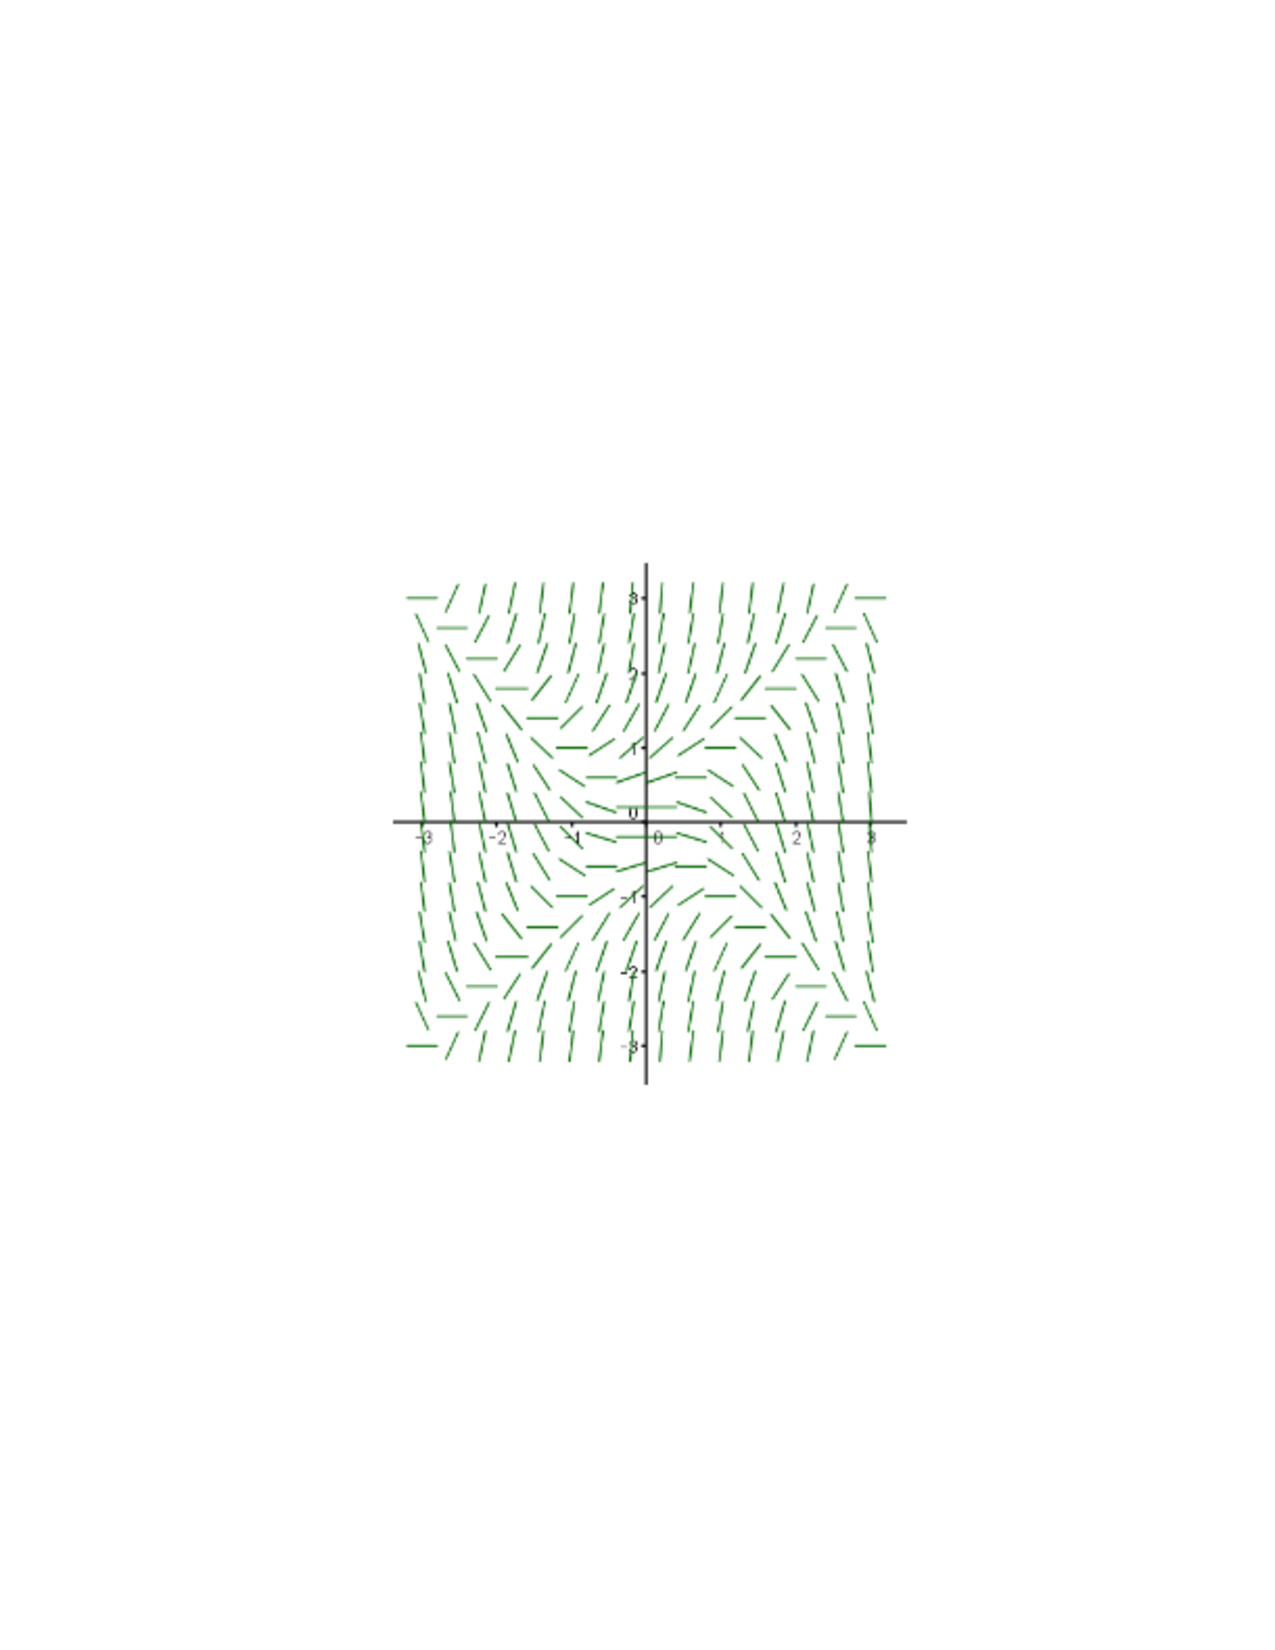
\includegraphics[trim= 300 280 250 280,scale=0.6]{Figure8-2-1.pdf}
		\end{image}
		
		Sketch the solution such that $y\left( \frac{1}{2} \right) = 1$.
	\begin{freeResponse}
	
	\begin{image}
	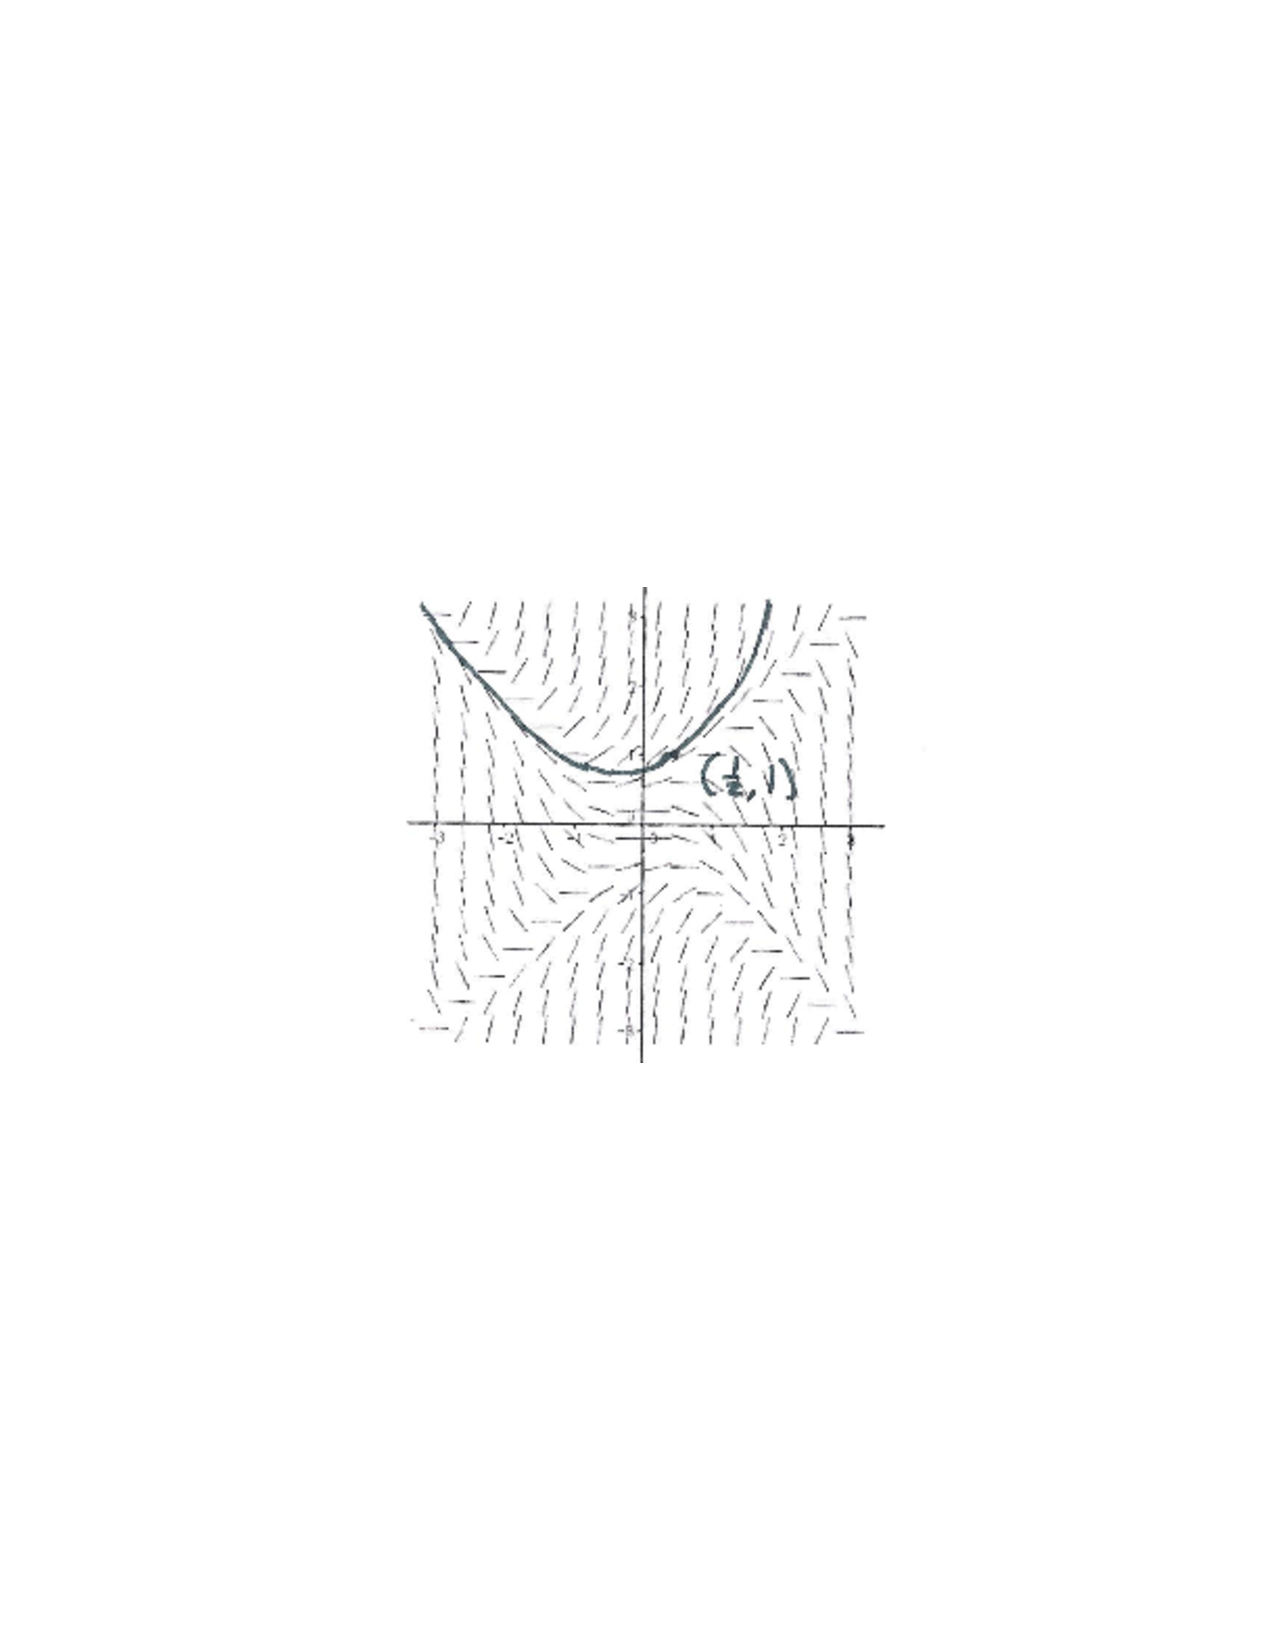
\includegraphics[trim= 330 260 250 300,scale=0.6]{Figure8-2-4.pdf}
	\end{image}
	
	\end{freeResponse}
	
	
\end{problem}

\begin{instructorNotes}
The major point here is that (a) and (b) are the same problem, presented with two different representations.
\end{instructorNotes}

%problem 2
\begin{problem}
Which of the following direction fields is the direction field corresponding to the differential equation $y' = 1+y^2$?

	
	\begin{image}
	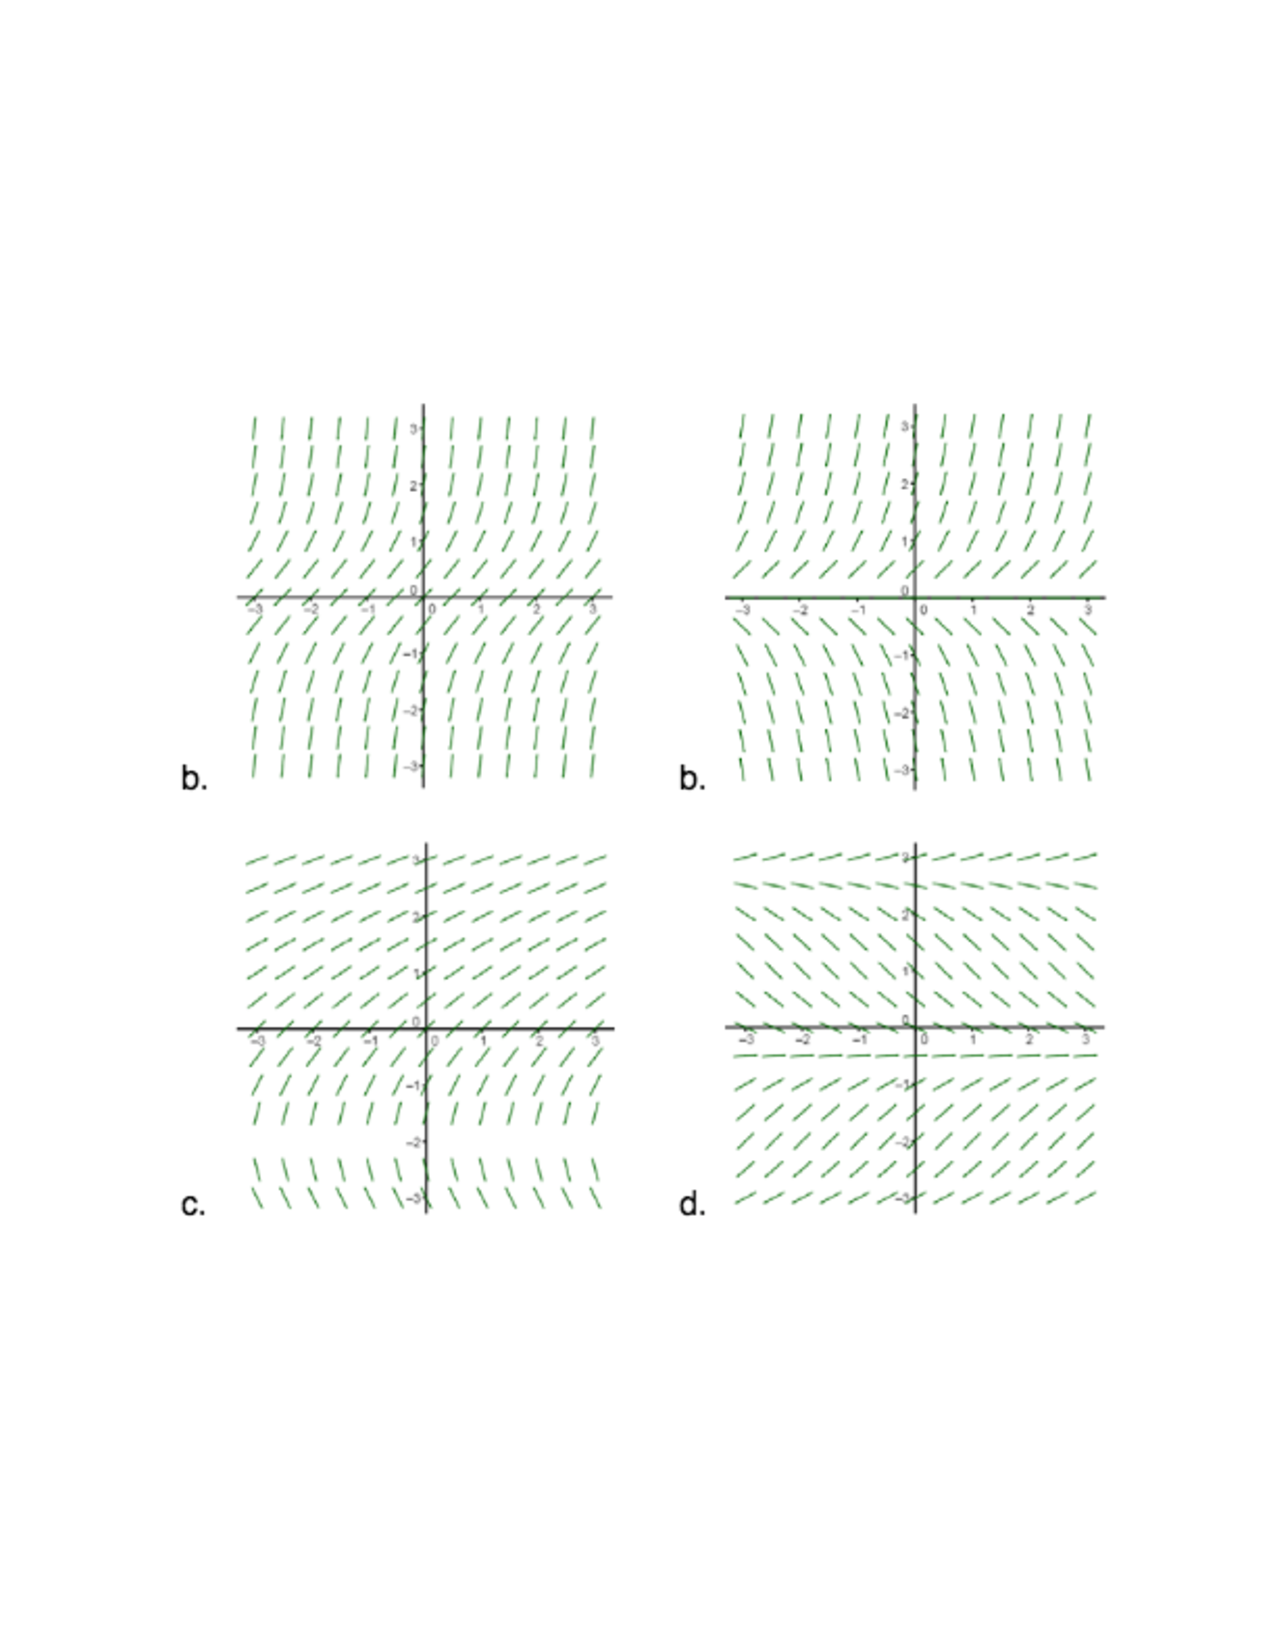
\includegraphics[trim= 250 200 250 200,scale=0.8]{Figure8-2-3.pdf}
	\end{image}
	
	\begin{freeResponse}
	Look along the line $t=0$ (the $y$-axis).

	Here $y' = 1+y^2$, so there is no $t$ on the right hand side of the equation.  
	Therefore, $y'$ depends only on $y$.  
	At $y=0$ the slope is $1$, then as $y$ increases the slopes increase too.  
	Similarly, as $y$ gets more and more negative, the slope gets more and more positive.  
	So it seems as if this direction field is (a).

	\end{freeResponse}

\end{problem}

\begin{instructorNotes}
Several strategies exist.  
Make sure to ask what special quality direction fields of autonomous differential equations have.  
Depending on time, this also could all be done as a whole class.
\end{instructorNotes}











	
	
	

	










								
				
				
	














\end{document} 


















